%****************************************************************************%
%* DIET User's Manual JXTA chapter file                                     *%
%*                                                                          *%
%*  Author(s):                                                              *%
%*    - Cedric TEDESCHI (Cedric.Tedeschi@insa-lyon.fr)                      *%
%*                                                                          *%
%* $LICENSE$                                                                *%
%****************************************************************************%



\chapter{P2P DIET extension}
\label{ch:p2pextension}

To extend the field of the available services for each client in a
transparent manner, DIET uses the Multi-Agent system to increase
scalability. To achieve this, the MAs access each others' resources
when processing a client's request. Thus, each request is not only
submitted inside the tree of the MA contacted by the client, but also
inside the tree of MAs connected to the first MA, if the first
submission failed.

\section{P2P and JXTA}
\label{sec:JXTA}

One way to implement the Multi-MA is to use peer-to-peer technology,
and thus have a distributed Multi-Agent system where MAs dynamically
discover each other and cooperate in order to give clients the largest
possible area of search.

JXTA~\cite{JXTA} is a technology written with java~\cite{java}. It
aims at allowing the development of destributed applications using
peer-to-peer concepts and the java language. JXTA provides
functionalities such as passing firewalls and similar network
protections, dynamically discovering other peers, and other essential
tools to develop a Multi-Agent system using peer-to-peer technology.

\section{Description of the current architecture developed with JXTA}
\label{sec:archi}

In this chapter we discuss \textbf{the first prototype}. We plan to
update this prototype with a future powerful Multi-MA using an
algorithm of discovery. The architecture of DIET/JXTA is shown Figure
7.1. We can consider that the elements allowing its use are divided in
two parts:

\begin{itemize}
\item{a JXTA part that includes client$_{JXTA}$, MA$_{JXTA}$ and
    SeD$_{JXTA}$. These components are written in java to be able to
    communicate together using JXTA.}
  
\item{a part of integration of the JXTA part in DIET: java (JXTA) and
    C++ (DIET) must cooperate. The technology used to allow this
    integration is JNI~\cite{JNI} that allows java to call functions
    written in C++. JNI is located in the MA and the SeD: The
    MA$_{JXTA}$ has to launch and communicate with a C++ MA$_{DIET}$.
    A similar interface appears in the SeD communication process.}
\end{itemize}

\begin{figure}[htb]
 \begin{center}
   \resizebox{.7\linewidth}{!}{\includegraphics{fig/global_platform_jxta.eps}}
  \label{fig:platform}
  \caption{DIET/JXTA architecture}
 \end{center}
\end{figure}

\subsection{The JXTA components}
\label{ssec:jxtacomponents}

\subsubsection{The client$_{JXTA}$}
\label{sssec:jxtaclient}

Only one component, the client, is fully written in java. Since it
communicates only with JXTA components, it doesn't need the DIET
client library.  JXTA pipes don't allow all types of data to be sent
through. The description of the problem and the problem itself have to
be packed to be sent through JXTA pipes. These messages are unpacked
inside the MA$_{DIET}$ and SeD$_{DIET}$.

The behaviour of the JXTA client is:

\begin {itemize}
\item{launch a new JXTA peer,}
\item{get MA$_{JXTA}$ advertisements (JXTA messages travelling through
    the network identifying a JXTA object) by sending a JXTA discovery
    query,}
\item{extract the reference of the input pipe of the first
    MA$_{JXTA}$ advertisement discovered,}
\item{create an output pipe to bind the input pipe extracted,}
\item{create and send the description of the problem via the pipe
    created and wait for the response of the MA$_{JXTA}$ connected,
    including references of SeDs able to solve the problem,}
\item{Try to create an output pipe to bind the input pipe of one of
    the SeDs found,}
\item{send the packed problem including data needed for the
    computation to the SeD bound and wait for its response,}
\item{Extract results of the response received.}
\end{itemize}

\subsubsection{The SeD$_{JXTA}$}
\label{sssec:jxtased}

The role of the SeD$_{JXTA}$ is to allow the clients$_{JXTA}$ to send
computation requests the SeD$_{DIET}$. The SeD$_{DIET}$ receives the
requests sent by clients$_{JXTA}$, calls the SeD$_{DIET}$ (that
returns the response),then sends the result to the client.

The general behaviour of the SeD$_{JXTA}$ is written below:

\begin{itemize}
  
\item{launch a new JXTA peer,}
\item{create an input pipe to receive the clients' requests,}
\item{launch the SeD$_{DIET}$,}
\item{process each request by a thread that:
\begin{itemize}
\item{forwards the packed request received to the SeD$_{DIET}$ and
    waits for a packed response,}
\item{sends the response to the client after having bound an output
    pipe to its input pipe.}
\end {itemize}}
\end{itemize}

\subsubsection{The Multi-MA$_{JXTA}$}
\label{sssec:jxtamultima}

The Multi-MA$_{JXTA}$ is composed of all MAs$_{JXTA}$ running at the
same time. The MA$_{JXTA}$ is able to connect the clients$_{JXTA}$ and
to others MA$_{JXTA}$ running at the same time. Thus, clients know
only one MA$_{JXTA}$, that is its access to the Multi-MA.  Each
MA$_{JXTA}$ publishes an advertisement with a lifetime in order to
avoid clients or other MA$_{JXTA}$ to connect to a stopped
MA$_{JXTA}$. When it receives a request coming from a client, the
MA$_{JXTA}$ submits the problem description to DIET via the
MA$_{DIET}$ it has itself launched. If the submission returns a DIET
failure, the MA$_{JXTA}$ searches other MAs$_{JXTA}$. Then, it
forwards the client's request to other MAs$_{JXTA}$. SeD references
thus collected are merged and sent to the client.

The general algorithm of the MA$_{JXTA}$ is as follows:

\begin{itemize}
\item{launch a new JXTA Peer,}
\item{build an input pipe to listen to client's requests or agent's
    forwarded requests,}
\item{create an advertisement including its input pipe reference
    allowing clients to connect it and publish it with a hardcoded
    lifetime,}
\item{process each client or agent message by a thread :
\begin{itemize}
\item{if the source of the message received is a client,}
  \begin{itemize}
  \item{call the MA$_{DIET}$ with the packed problem and get SeD
      reference(s),}
  \item{if any, send it to the client, else search other MA$_{JXTA}$,
      forward the query to the other MA(s)$_{JXTA}$ discovered and
      send a response containing all SeD references thus received to
      the client.}
  \end{itemize}
\item{if the source is an agent,}
          \begin{itemize}
          \item{call the MA$_{DIET}$ on the problem received and
              get SeD references found in its DIET tree, }
          \item{send a response including SeD reference(s) to the
              MA$_{JXTA}$ from which it received the request.}
          \end{itemize}
\end{itemize}}
\end{itemize}

\subsection{The DIET/JXTA interface: JNI}
\label{ssec:jni}

JNI is a technology allowing programmers to call native methods
(written in C/C++) from a program written in java. As seen before, the
DIET/JXTA components having a DIET part and a JXTA part are the MA
and the SeD.

\subsubsection{The MA$_{DIET}$}
\label{sssec:jnima}

To submit the client's requests to DIET, the MA$_{JXTA}$ has to call the MA$_{DIET}$ 
\texttt{submit} function. To allow this, the MA$_{JXTA}$ launches a MA$_{DIET}$ via a 
native method and calls the \texttt{submit} function via another.

The MA$_{DIET}$ contains:

\begin{itemize}
\item{a native method that launches the MA$_{DIET}$,}
\item{a native method \texttt{submitJXTA} that:}
\begin{itemize}
\item{unpacks the description of the problem to be solved in order to
    build a DIET problem description,}
\item{calls the DIET \texttt{submit} function and thus gets a
    response,}
\item{extracts and returns the SeD reference(s) to the MA$_{JXTA}$.}
  \end{itemize}
\end{itemize}

\subsubsection{The SeD$_{DIET}$}
\label{sssec:jnised}

To solve the client's computation requests, the SeD$_{JXTA}$ needs to
call the SeD$_{DIET}$ \texttt{solve} function. In the same manner as
above, to allow this, the SeD$_{JXTA}$ launches the SeD$_{DIET}$ via a
native method, and calls the \texttt{solve} function via another.

The SeD$_{DIET}$ contains:

\begin{itemize}
\item{a native method that launches the SeD$_{DIET}$,}
\item{a native method \texttt{solveJXTA} that:}
        \begin{itemize}
        \item{unpacks the problem to be solved and builds a DIET
            profile,}
        \item{calls the \texttt{solve} function,}
        \item{extracts and returns the response to the SeD$_{JXTA}$.}
        \end{itemize}
\end{itemize}

\section{The future of DIET/JXTA}
\label{sec:future}

\subsection{Remaining problems}
\label{ssec:remainingpbs}

\begin{itemize}
\item{An unsolved problem dealing with \textbf{omniORB and JNI}
    results in a failure when a JNI SeD$_{DIET}$ registers to a DIET
    Agent not launched via JNI. Because of that, to deploy some LAs
    between a DIET/MA$_{JXTA}$ and a DIET/JXTA SeD, they have to be
    launched via JNI.  Moreover, a DIET/MA$_{JXTA}$ won't be able to
    know LAs or SeDs not launched via JNI.  The current DIET/JXTA tree
    is unable to contain classic LAs$_{DIET}$ or SeDs$_{DIET}$.}
  
\item{The current version of the DIET/JXTA platform works only for
    problems having two input matrices and one output matrix. The
    serialization has been written only for these cases. One of the
    first things to do is to write a \textbf{generic packing and
      unpacking}, to be able to process all problems supported
    by DIET.}

\end{itemize}

\subsection{Next developments}
\label{ssec:nextdev}

\begin{itemize}
\item{The client$_{JXTA}$ isn't very simple to write, because nothing
    is hidden, neither the details of the JXTA communication nor the
    creation of the problem. As for the client$_{DIET}$, an API
    providing all mechanisms needed to communicate with DIET via JXTA
    pipes should be written. The implementation of a Java Client
    taking in account the JXTA communication seems to be the
    solution.}
  
\item{The current algorithm of the Multi-MA is a sequential one. When
    a MA$_{JXTA}$ forwards a request, the other MA(s)$_{JXTA}$ are
    contacted one by one, in the order they have been discovered by
    JXTA. This algorithm will be replaced by a real discovery
    algorithm. Moreover, for now, the discovery is made within the
    entire JXTA net peer group, what makes the discovery impractical
    when getting out of the local network. The MA$_{JXTA}$ will have
    its own peer group in the future in order to optimize the
    discovery.}
\end{itemize}


\section{Working with a DIET/JXTA platform}
\label{sec:workwithjxta}

\subsection{Installation and configuration}
\label{ssec:installjxta}

\begin{itemize}
\item{Download the JDK1.4.1 or later release from for instance:
    \texttt{http://java.sun.com/\linebreak[4]j2se/1.4.2/download.html}
    (Previous JDKs are known to generate errors with JXTA 2.0) and set
    environment variable PATH with java binaries location.}
\item{Download from
    \texttt{http://download.jxta.org/stablebuilds/index.html} and
    extract the JAR files of the last stable JXTA release (current
    version of DIET/JXTA is based on JXTA 2.3). Files to download are
    :}
\begin{itemize}
\item{\texttt{jxta.jar},}
\item{\texttt{jxtasecurtity.jar},}
\item{\texttt{jxtalib.zip},}
\item{\texttt{jxtaext.zip}.}
  \end{itemize}
  
\item{Unzip the ZIP files and set environment variable named
    \texttt{JXTA\_LIB} containing the directory where you extracted
    the JAR files.}
  
\item{Then, to configure DIET and to deploy DIET/JXTA platforms, the
    \texttt{./configure} command must be run with options including
    \texttt{--enable-JXTA-mode} (warning, case sensitive!) and
    �\texttt{--enable-examples} for the client$_{JXTA}$. It is
    recommended to add the option \texttt{--without-FAST}, because no
    scheduling is made in the current DIET/JXTA platform.}

\end{itemize}

\subsection {Deploying a DIET/JXTA platform}
\label{ssec:deployjxta}

Please refer to the previous chapter for more information concerning
things to do before deploying the platform.

\begin {itemize}
\item{\textbf{First step}: launching a MA$_{JXTA}$. After having set the
    \texttt{OMNIORB\_CONFIG} and \\ \texttt{OMNINAMES\_LOGDIR} paths, DIET is ready
    to run, except the JXTA part. You have to set : }

    \begin{itemize}
    \item {\texttt{LD\_LIBRARY\_PATH}, to allow the java classes to load
        libraries including the native methods : \\ \texttt{<DIET\_root>/src/agent/.libs}.}
    \item{\texttt{JXTA\_LIB}, the directory containing the JXTA JARs,}
    \item{At last, the command to be launched to run a MA$_{JXTA}$ is:\\\\
        \texttt{\$ java -cp <JXTA\_JARS> JXTAMultiMA <DIET\_MA\_config\_file>}\\\\
        Ensure that this command is launched inside the right
        directory : indeed, only one peer can be launched by directory
        : information concerning this peer is available in a
        \texttt{.jxta} directory under the directory where you
        launched the peer.  Delete this directory before launching a
        peer if you have already used it on another machine, in order
        to clean the platform configuration.}
  
    \item{Each time a new JXTA peer is launched, you have to configure
        it.  On the first setup screen, the name of the peer is
        required and must be unique, for instance, ``MA1''. The second
        screen, named ``advanced'', displays the TCP and HTTP
        settings. When using DIET/JXTA on a single machine, the
        configuration is on figure 7.2, in the other case, just
        replace \texttt{localhost} by the IP address of the machine.
        Please note that, for each peer on a single machine, the TCP
        and HTTP ports have to be different. For instance : 9701 and
        9700 for the first peer, 9703 and 9702 for the second, ... The
        third setup screen deals with the web access. If you want to
        access peers outside the local network, references of
        rendezvous and relay peers placed at the disposal of JXTA
        users by the JXTA developpers can be downloaded. Otherwise,
        don't do anything with this screen. The last screen deals with
        username and password, but these parameters are filled with
        default values.}
    \end{itemize}

\begin{figure}[htb]
 \begin{center}
  \resizebox{.7\linewidth}{!}{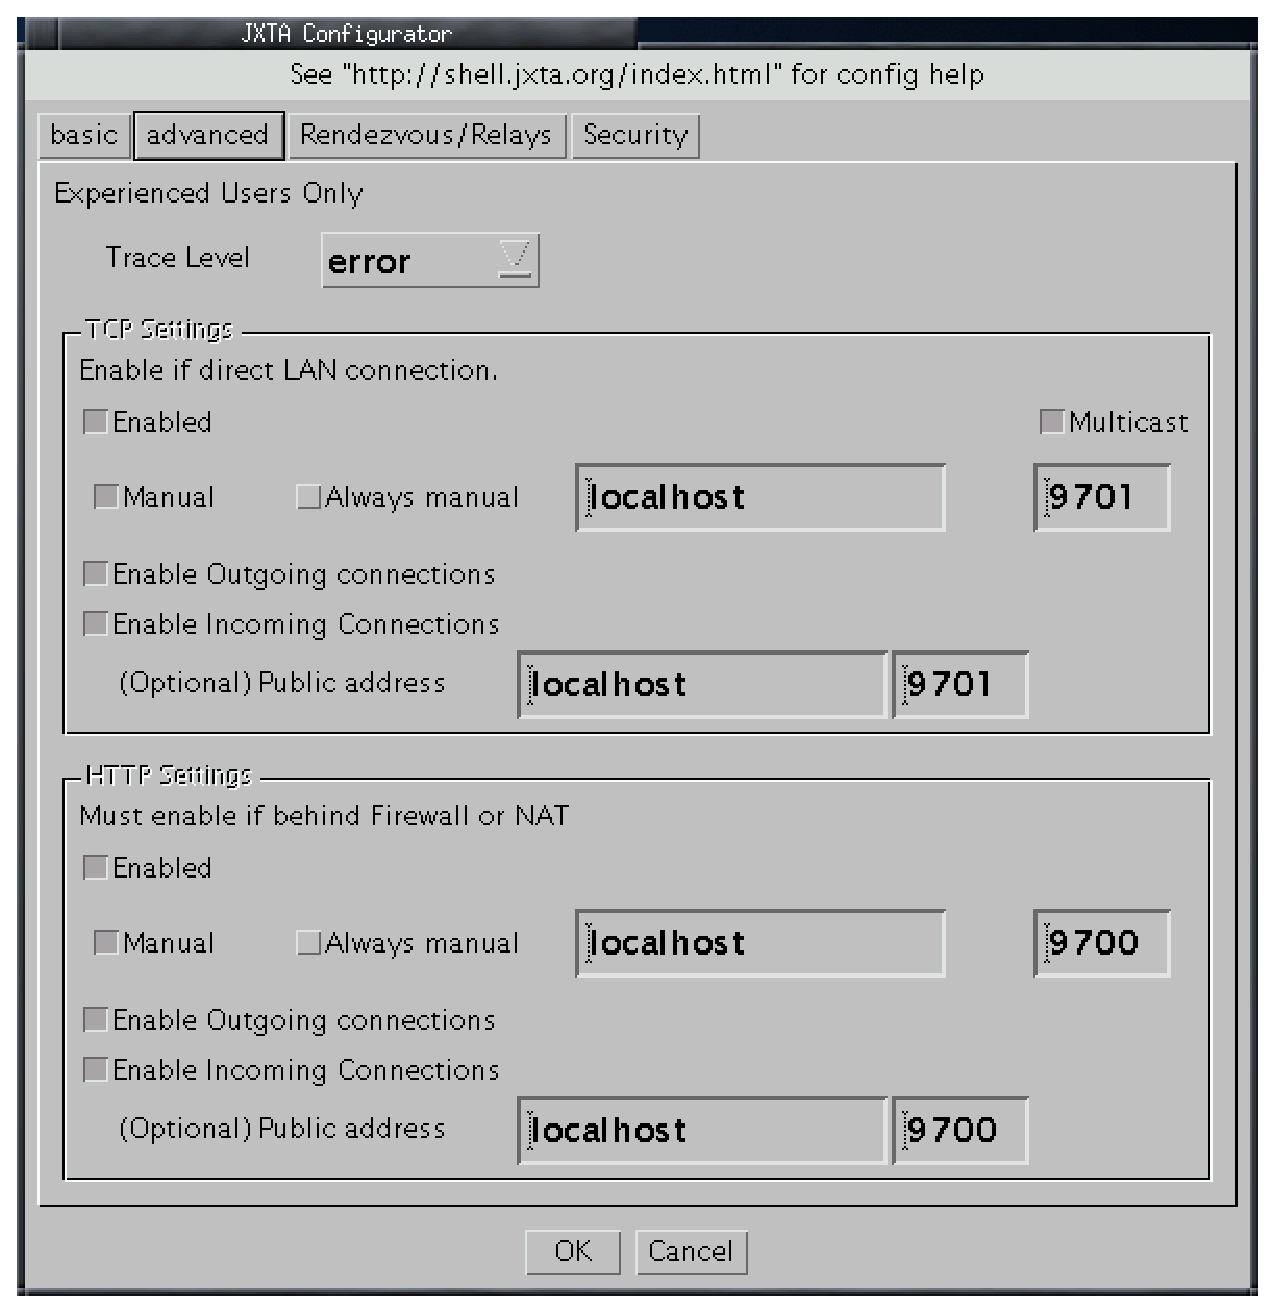
\includegraphics{fig/JXTAConfig.ps}}
  \label{fig:platform}
  \caption{General architecture of DIET/JXTA}
 \end{center}
\end{figure}

\item{\textbf{Second step}: registering a SeD to the MA. The same
    paths must be set:\\ (\texttt{<DIET\_root>/src/SeD/.libs} for
    \texttt{LD\_LIBRARY\_PATH}.) Be sure that the \texttt{parentName}
    inside the configuration file matches the name
    of the MA$_{DIET}$ previously launched. The command to run is:\\\\
    \texttt{\$ java -cp <JXTA\_LIBS> JXTASeD
      <DIET\_SeD\_config\_file>\linebreak[4] <computation\_abilities>}
    \\\\ If you want to put LA(s) between the MA and the
    SeD, launch the following command before loading the SeD:\\\\
    \texttt{\$ java LA <DIET\_LA\_config\_file>}\\\\ Check the DIET
    tree coherence and the \texttt{parentName} variables inside the
    configuration files. }

\item{\textbf{Third step}: Launch a JXTA client with the command:\\\\
                    \texttt{\$ java -cp <JXTA\_LIBS> ClientJXTA <pb>}}

\end{itemize}

At this point, you still haven't tested the Multi-MA. To achieve this,
launch other MA$_{JXTA}$(s) and launch again the client.

Scripts have been left at your disposal. You just need to check the
environment variables and paths required. As said before, only one
JXTA peer can be run in one directory, so each script is inside a
different one. These directories have to be edited (for configuration), are named
\texttt{MMA1/}, \texttt{MMA2/}, \texttt{MMA3/}, \texttt{LA1/},
\texttt{SeD1/}, \texttt{SeD2/} and \texttt{client/}.  and are located
in : \texttt{<DIET\_root>/src/example/jxta/scripts}.
 

